\documentclass[fontsize=11pt]{article}
\usepackage{amsmath}
\usepackage[utf8]{inputenc}
\usepackage[margin=0.75in]{geometry}
\usepackage{listings}
\usepackage{xcolor}
\usepackage[T1]{fontenc}
\usepackage{url}

\usepackage{graphicx}
\usepackage[
  backend=biber,
  style=ieee,
  sorting=ynt
]{biblatex}
\addbibresource{assets/main.bib}

\lstset{
  language=Python,
  basicstyle=\small\ttfamily,
  columns=fullflexible,
  showstringspaces=false,
  breaklines=true,
  keywordstyle=\color{blue}\bfseries,
  commentstyle=\color{gray},
  stringstyle=\color{teal},
  numbers=left,
  numberstyle=\tiny\color{gray},
  frame=single
}

\title{CAN-GAT: Drug Target Interaction Prediction for Molecular Cancer Drugs Employing Graph Attention Networks}
\author{Albert Guo, Adarsh Padalia, Yunzhe Qiao, Mark Wang}
\date{Wednesday, March 27, 2025}
\begin{document}
\maketitle
\begin{abstract}
Cancer is currently the leading cause of death in Canada \cite{CCS2021}, and a leading cause of death worldwide \cite{Sung2021}. Despite its prominence, cancer remains difficult to treat in part due to the similarity between cancer cells and healthy cells. Targeted molecular therapies have shown promise, designed to be able to bind specifically to proteins that cancers use to signal and replicate. The first targeted cancer drug, imatinib, was approved in 2001 and has shown significant efficacy against chronic myelogenous leukemia (CML) \cite{Druker2001}. Since then, other targeted therapies, such as those for treating epidermal growth factor receptor positive non-small cell lung carcinoma (EGFR+ NSCLC) \cite{Rosell2012}, have been developed. Many of these therapies are highly effective; however, substantial barriers to the discovery of these targeted therapies remain. In particular, predicting specific drug-target interactions is challenging due to the complex nature of these interactions, which depend on the amino acid sequence of the protein, its folded structure, and the molecular structure of the drug candidate. In this paper, we analyze the use of a novel Graph Attention Network (GAT) \cite{Velickovic2018} for assessing drug-target interaction predictions on the CandidateDrug4Cancer dataset \cite{Ye2022}. We were able to achieve significant improvements over the existing DTI prediction models, such as those employing Morgan fingerprints \cite{Rogers2010} combined with XGBoost \cite{ChenGuestrin2016}, and we believe that our model shows significant promise for the complex field of drug discovery.
\end{abstract}

\section*{Introduction}

Drug-Target Interaction (DTI) prediction has long been recognized as a critical step in the drug development pipeline \cite{Chen2016}. Traditionally, this process relied heavily on experimental screening, which was both time-consuming and costly. In recent years, advances in artificial intelligence (AI) have introduced new approaches for accelerating drug discovery. Among these, Graph Neural Networks (GNNs) have emerged as a powerful tool capable of leveraging the structural information inherent in molecular graphs \cite{Velickovic2018}.

In this study, we focused on the CandidateDrug4Cancer dataset \cite{Ye2022}, which included 29 cancer-associated protein targets, 54,869 drug molecules, and 73,770 known drug-protein interactions. Each molecule was represented as a graph, where nodes corresponded to atoms and edges represented chemical bonds. Our primary task was to predict the likelihood of a biological interaction between a given drug and a cancer target protein based on this structural data.

We implemented a Graph Attention Network (GAT) using PyTorch \cite{Velickovic2018} to perform DTI prediction and compared its performance to traditional baseline methods, such as Morgan fingerprints \cite{Rogers2010} combined with XGBoost \cite{ChenGuestrin2016}. We also visualized the model’s output using Feature Activation Maps \cite{Pope2019} to interpret the predicted efficacy of specific drugs. The objective was to assess whether GATs could offer improved accuracy and predictive insight over conventional approaches in the context of cancer-targeted drug screening.

\section*{Computational Overview}

To implement this, we divide the computing process into the following steps: Data Processing, Graph Construction, Neural Network Model Architecture, Training Process, Evaluation, and Hyperparameter Tuning and Optimization.
\begin{itemize}
    \item \textbf{Data Processing} \subsubsection*{1.\quad Dataset Structure}
Typically, each row in the interaction table provides the following columns:

\begin{center}
\begin{tabular}{|l|l|p{9cm}|}
\hline
\textbf{Column}       & \textbf{Type}    & \textbf{Description} \\
\hline
\texttt{ChEMBL\_ID} & String           & ChEMBL identifier of the compound (e.g., \texttt{CHEMBL123456}). \\
\texttt{Target\_ID}   & String           & ChEMBL identifier of the target (e.g., \texttt{CHEMBL1824}). \\
\texttt{pChEMBL\_Value} & Float         & $-\log_{10}$ of the measured IC\textsubscript{50}. \\
\texttt{SMILES}       & String           & Chemical structure in SMILES format. \\
\texttt{Protein}    & String            & Full amino acid sequence of the target protein. \\
\texttt{Label} & Boolean & Binary indicator of active/inactive \\
\hline
\end{tabular}
\end{center}

\subsubsection*{2.\quad Equations for Label Computation and Molecular Features}

\begin{quote}

    \textbf{2.1 pChEMBL and Activity Label}
    
    \quad The dataset leverages a $p\text{ChEMBL}$ value, defined by:
    \[
        p\text{ChEMBL} \;=\; -\log_{10}\bigl(\text{IC}_{50} \text{ in molar}\bigr),
    \]
    which transforms IC\textsubscript{50} from molar units into a logarithmic scale. 
    
    A threshold $\texttt{pChEMBL} \ge 7.0$ (corresponding to IC\textsubscript{50} $\leq 100\text{ nM}$) 
    denotes a \emph{potent} interaction. Hence, we define the activity label as:
    
    \[
        \text{Activity\_Label} \;=\; 
        \begin{cases}
        1, & \text{if } p\text{ChEMBL} \ge 7.0,\\
        0, & \text{otherwise}.
        \end{cases}
    \]
    
    \textbf{2.2 Molecular Graph Features}
    
    \quad For each molecule, we parse the SMILES string into a graph. Let $V = \{v_1, v_2, \dots, v_n\}$ 
    be the set of atoms, and $E = \{(v_i, v_j)\,\mid\, \text{bond exists between }v_i \text{ and } v_j\}$ the set of edges. \\
    
    Each atom node $v_i$ has features such as:
    \begin{quote}
        \begin{itemize}
            \item[1.] \emph{Atom Type} (atomic number)
            \item[2.] \emph{Formal Charge}
            \item[3.] \emph{Degree} (number of covalent bonds to $v_i$)
            \item[4.] \emph{Hybridization} (e.g., sp, sp2, sp3)
            \item[5.] \emph{Aromaticity}
        \end{itemize}
    \end{quote}
    Each bond $(v_i, v_j)$ has features like:
    \begin{quote}
        \begin{itemize}
            \item[1.] \emph{Bond Type} (Single, Double, Triple, Aromatic)
            \item[2.] \emph{Conjugation}
            \item[3.] \emph{Ring Membership}
        \end{itemize}
    \end{quote}

\end{quote}

\subsubsection*{3.\quad Data Preprocessing and Splitting}

\begin{quote}
    \textbf{Step 1: Loading Data.} We first read the CSV file that contains the compound--target interactions:
    \begin{lstlisting}[language=Python]
    import pandas as pd
    
    df = pd.read_csv("CandidateDrug4Cancer_full.csv") 
    print(df.head())
    \end{lstlisting}
    
    \noindent
    \textbf{Step 2: Creating Activity Labels.} If the label is not already present, we define:
    \begin{lstlisting}[language=Python]
    df["Activity_Label"] = (df["pChEMBL_Value"] >= 7.0).astype(int)
    \end{lstlisting}
    
    \noindent
    \textbf{Step 3: Splitting into Train/Validation/Test.} We split randomly or by target:
    \begin{lstlisting}[language=Python]
    from sklearn.model_selection import train_test_split
    
    train_df, temp_df = train_test_split(df, test_size=0.3, stratify=df["Activity_Label"])
    val_df, test_df   = train_test_split(temp_df, test_size=0.5, stratify=temp_df["Activity_Label"])
    \end{lstlisting}
\end{quote}

\subsubsection*{4.\quad Graph Construction (Feature Computation)}
Using RDKit, we convert each SMILES to a molecule and extract the heavy-atom graph:
\begin{lstlisting}[language=Python]
from rdkit import Chem
from typing import Any

def construct_molecular_graph(smiles_str: str) -> dict[str, list[Any]]:
    mol = Chem.RemoveHs(Chem.MolFromSmiles(smiles_str)) # remove explicit H atoms

    node_features = []
    adjacency_list = []
    edge_features = []

    for atom in mol.GetAtoms():
        feats = {
            "atomic_num": atom.GetAtomicNum(),
            "formal_charge": atom.GetFormalCharge(),
            "degree": atom.GetDegree(),
            "hybridization": str(atom.GetHybridization()),
            "aromatic": int(atom.GetIsAromatic())
        }
        node_features.append(feats)

    for bond in mol.GetBonds():
        i = bond.GetBeginAtomIdx()
        j = bond.GetEndAtomIdx()
        bond_feat = {
            "bond_type": str(bond.GetBondType()),
            "conjugated": int(bond.GetIsConjugated()),
            "ring": int(bond.IsInRing())
        }
        edge_features.append(((i,j), bond_feat))
        % Undirected adjacency
        adjacency_list.append((i, j))
        adjacency_list.append((j, i))

    return {
        "node_features": node_features,
        "edge_features": edge_features,
        "adjacency_list": adjacency_list
    }
\end{lstlisting}

\noindent
\emph{Explanation:} We record atom-level descriptors (atomic number, formal charge, etc.) and 
bond-level descriptors (bond type, conjugation, ring membership). The adjacency list is built
from each bond pair (i, j). This structure can be fed into a graph neural network or converted 
into other GNN frameworks like PyTorch Geometric or DGL.

\item \textbf{Construct Graph Attention Network (GAT)}: The Graph Attention Network architecture first processes each drug’s molecular graph through multiple GAT layers. Within each GAT layer, a node updates its embedding by computing attention scores for its neighbors. These scores highlight the relative importance of different neighboring nodes, and multi-head attention further stabilizes learning by combining insights from multiple parallel attention mechanisms \cite{Velickovic2018}. After the message passing phase, a pooling operation generates a single embedding for the entire molecule, typically by taking a mean or weighted sum of node embeddings. The final output of the GAT model is the predicted pChEMBL for the drug-protein pair. \\
    
    \small \textbf{Remark: Graph Attention Network Equations}

    \begin{itemize}
            \item[$\circ$] \textbf{Attention Coefficients:} For each node $i$, we compute attention scores $a_{ij}$ toward each neighbor $j$ as follows:
            \[
                \alpha_{ij} \;=\;
                \frac{\exp\!\Bigl(\mathrm{LeakyReLU}\bigl(\mathbf{a}^\mathsf{T}
                    \bigl[\mathbf{W}\mathbf{h}_i \,\|\, \mathbf{W}\mathbf{h}_j\bigr]\bigr)\Bigr)}
                     {\sum_{k \in \mathcal{N}(i)} \exp\!\Bigl(\mathrm{LeakyReLU}\bigl(\mathbf{a}^\mathsf{T}
                       \bigl[\mathbf{W}\mathbf{h}_i \,\|\, \mathbf{W}\mathbf{h}_k\bigr]\bigr)\Bigr)},
            \]
            where $\mathbf{h}_i$ is the current feature vector for node $i$, $\mathbf{W}$ is a trainable weight matrix, and $\mathbf{a}$ is a learnable vector for the attention mechanism \cite{Velickovic2018}.

            \item[$\circ$] \textbf{Node Representation Update:} After normalizing coefficients, we update the node representation: 
            \[
                \mathbf{h}_i' \;=\;
                \sigma\!\Bigl(\sum_{j \in \mathcal{N}(i)}
                      \alpha_{ij}\,\mathbf{W}\,\mathbf{h}_j\Bigr),
            \]
            where $\sigma$ is a non-linear activation function (ReLU in our case) \cite{Velickovic2018}.
        \end{itemize}

    \item \textbf{Training Process}: Training was preformed on an Nvidia A5000 (Ampere) GPU. During training, the model uses Huber loss to predict whether a drug-protein pair is likely to bind. The Adam optimizer updates the network parameters, and regularization methods, such as dropout and weight decay, help the network generalize better. Early stopping is employed by monitoring the validation loss and halting training when performance ceases to improve, which avoids excessive overfitting \cite{Chen2016}.\\

    \item \textbf{Evaluation}
    \begin{itemize}
        \item[1.] Our study compared the GAT-based approach against a baseline model that uses Morgan fingerprints \cite{Rogers2010} to encode drug molecules. In the baseline method, circular fingerprints capture substructures around each atom, and a gradient boosting algorithm, XGBoost \cite{ChenGuestrin2016}, processes these representations together with simpler protein features. By evaluating the two approaches side by side, we assess whether the structural awareness introduced by graph neural networks provides a significant performance boost over traditional fingerprint-based techniques.
        \item[2.] Model performance is evaluated using multiple metrics to capture different aspects of prediction quality. Since this is a prediction algorithm and not a classification algorithm, we define the prediction as correct when:
        \[
        |\textit{predicted ChEMBL score} - \textit{actual pChEMBL score}| < 1.0
        \]
        and define the accuracy as:
        \[
        \frac{\textit{number of correct predictions}}{\textit{number of samples}}.
        \]
        Additionally, we evaluate the model in terms of mean absolute error (MAE) and mean squared error (MSE) \cite{Chen2016}.
        
        \quad An object-oriented Graph class is implemented to simplify the process of storing and retrieving molecular structures. This class keeps track of adjacency lists, node features, and bond attributes, and offers methods for adding nodes, adding edges, and retrieving neighbor information \cite{Chen2016}.

        \quad In addition, the \texttt{GATModel} class encapsulates the GAT layers, along with a residual connection and a fully connected layer for the final prediction. It provides a \texttt{forward(drug\_graph, protein\_embedding)} method returning an interaction probability. A \texttt{Trainer} class is also implemented to coordinate the training loop, including batch processing, loss computation, backpropagation, and metric logging \cite{Chen2016}.
    \end{itemize}

    \item \textbf{Hyperparameter Tuning}: Hyperparameter tuning explores a range of values for the learning rate, hidden dimension, attention heads, and dropout rates. A systematic approach, such as grid search or Bayesian search, helps identify settings that maximize validation performance while preserving generalization \cite{Kanakala2023}. Additional experiments can examine how the number of GAT layers affects the model’s ability to capture higher-order structural relationships within each molecule.
    
    \item \textbf{Visualizing the Results}: Upon training a successful model, we can determine the specific nodes and edges of the drug molecule that improve or impair the drug's efficacy using Feature Activation Maps \cite{Pope2019}. For example, given a drug/protein pair, we construct a graphical representation of the drug molecule (using a library like \texttt{networkx}) that utilizes color to show the relative contribution of different atoms and bonds to the efficacy of the drug \cite{Pope2019}.
    
\end{itemize}

\begin{lstlisting}[language=Python, caption={Python implementation of a Graph class for molecular data}, label={lst:graph_class}]
class Graph:
    """
    A Graph class to represent a molecular graph with atom-level and bond-level features.

    Instance Attributes:
        - neighbors: A dictionary mapping node IDs to a list of neighboring node IDs.
        - node_features: A dictionary mapping node IDs to a dictionary of that node's features.
        - edge_features: A dictionary mapping (node_i, node_j) to a dictionary of bond-level features.
    """
\end{lstlisting}

\begin{lstlisting}[language=Python, caption={Scratch implementation of \texttt{GATModel} and \texttt{Trainer} classes}, label={lst:listing2}]
class GATModel:
    """
    A model class containing the multi-head GAT architecture and downstream fully connected layers for final prediction.
    
    Instance Attributes:
        - num_heads: Number of attention heads.
        - hidden_dim: Dimensionality of the hidden layers.
        - gat_layers: A collection of GAT layers.
        - fc_layers: Fully connected layers to combine graph embeddings with protein features for final prediction.
    """


class Trainer:
    """
    A class used for coordinating the training loop, including data loading, backpropagation, and logging.
    
    Instance Attributes:
        - model: The GAT-based model to be trained.
        - optimizer: The optimizer used for parameter updates.
        - criterion: The loss function for computing training loss.
        - metrics: A collection of metric functions for evaluation.
        - device: The device (CPU or GPU) on which training is performed.
    """
\end{lstlisting}
\section*{Running the Model}
Ensure you have \verb|python 3.13| installed. To run the model, from the base directory, run:\\
\verb|pip install -r requirements.txt|\\
\verb|python main.py|\\

Note that \verb|tkinter| has known stability and compatibility issues on macOS, as the Apple-supplied python installation does not work well with \verb|tkinter|. If you are using an Apple Silicon device, you may need to reinstall Python from the official Python website or attempt to run the program on a different device.\\

Also know that PythonTA has issues running in some files. This is likely due to a bug within PythonTA, and how it interacts with other modules. 

\section*{Results}
Our model was able to significantly outperform the baseline Morgan Fingerprint technique \cite{Rogers2010,ChenGuestrin2016}, and was able to accurately predict the pChEMBL scores of several drugs. On the testing dataset, we achieved achieving a MAE of 0.540, and a $\pm1$ accuracy of 0.844. On the testing dataset, we achieved $\pm 1$ accuracy of $84.4\%$, meaning that $84.4\%$ of predictions by the model were within $\pm 1$ of the actual pChEMBL score. This indicates that our model is able to accurately predict the activity of the majority of molecular cancer drugs. In addition, our model was able to achieve an AUC of 0.901, which is extremely high.

\begin{figure}
    \centering
    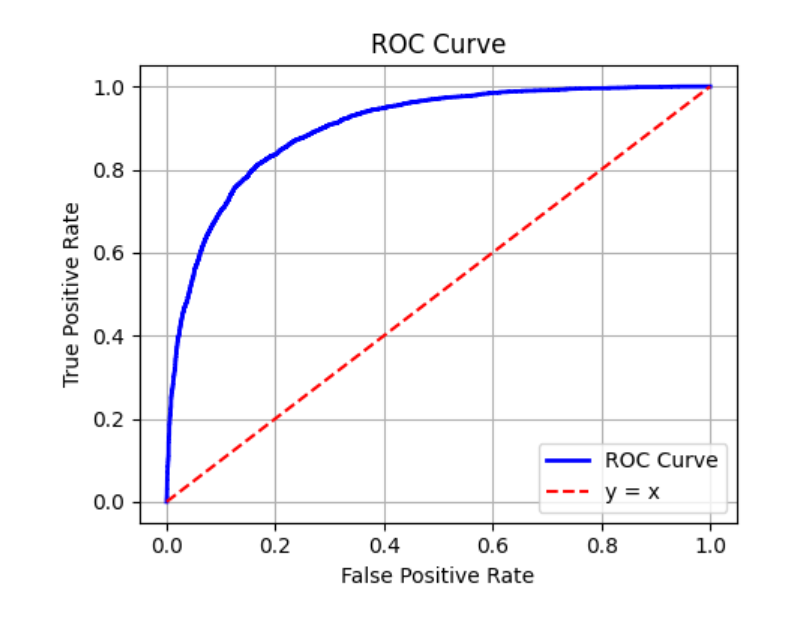
\includegraphics[width=0.5\linewidth]{assets/auc.png}
    \caption{AUC curve of model on testing data.}
    \label{fig:enter-label}
\end{figure}


\begin{table}[h]
    \centering
    \begin{tabular}{|c|c|c|c|c|c|}
        \hline
        Model & $\pm 1$ Accuracy & MSE & MAE & $R^2$ & AUC \\ \hline
        \textbf{CAN-GAT} & \textbf{0.844} & \textbf{0.540} & \textbf{0.551} & \textbf{0.645} & \textbf{0.901} \\ \hline
        Morgan Fingerprints + XGBoost & 0.741 & 0.779 & 0.707 & 0.484 & 0.746 \\ \hline
    \end{tabular}
    \caption{Performance metrics for different models}
    \label{tab:performance_metrics}
\end{table}

\begin{figure}
    \centering
    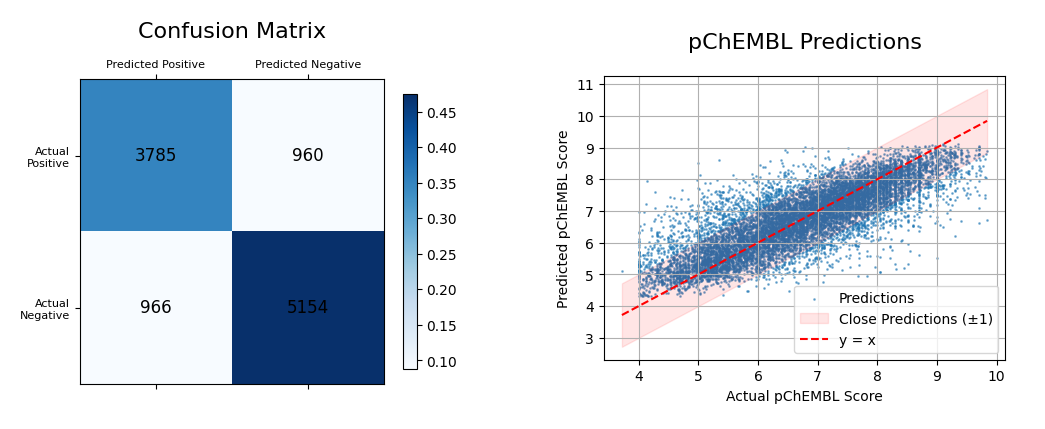
\includegraphics[width=1\linewidth]{assets/matrix+scatterplot.png}
    \caption{Confusion Matrix and scatterplot of model predictions on testing data.}
    \label{fig:enter-label}
\end{figure}

\begin{figure}
    \centering
    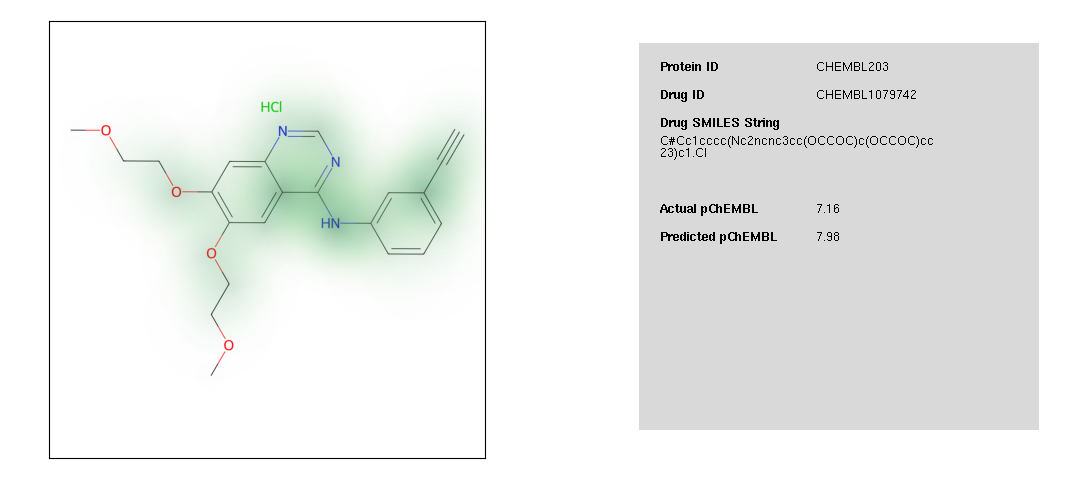
\includegraphics[width=1\linewidth]{assets/Erlotinib.png}
    \caption{Our model's prediction of Erlotinib's (Tarceva) activity, a commonly used epidermal growth factor receptor (EGFR) inhibitor used in treating non-small cell lung carcinoma (NSCLC) and pancreatic adenocarcinoma (PDAC) \cite{Rosell2012}. Green areas positively contribute to the predicted score; red areas negatively contribute to the predicted score.}
    \label{fig:enter-label}
\end{figure}

\section*{Discussion}
Our CAN-GAT model demonstrated promising performance in predicting drug-target interactions on the CandidateDrug4Cancer dataset \cite{Ye2022}. Compared to the baseline approach using Morgan fingerprints with XGBoost \cite{Rogers2010,ChenGuestrin2016}, CAN-GAT achieved lower MAE and MSE, and higher $\pm1$ accuracy, suggesting improved discrimination between active and inactive drug-target pairs. When benchmarked against other graph-based DTI prediction models, CAN-GAT aligns closely with approaches like those proposed by Veličković et al. \cite{Velickovic2018}. Unlike traditional cheminformatics methods that rely on fixed molecular descriptors, CAN-GAT leverages the full graph structure, offering a more flexible representation of chemical interactions. We aim to further refine our model and test against other state-of-the-art approaches such as the one proposed by Tsubaki et al. \cite{Tsubaki2019}.

Visualization of attention weights through Feature Activation Maps \cite{Pope2019} provided valuable insights into the molecular basis of drug efficacy. Generally speaking, amine functional groups and rings had high activation scores, indicating that they were especially important in determining the activity of compounds. These findings align with known principles of medicinal chemistry \cite{Chen2016} and could help to make our model more interpretable, rather than simply being a "black box" prediction model.

Despite its strengths, CAN-GAT faces several limitations. The CandidateDrug4Cancer dataset, while comprehensive, includes only 29 cancer-associated protein targets, potentially limiting the model's ability to generalize across diverse protein families \cite{Ye2022}. Additionally, the computational complexity of multi-head attention mechanisms increases training time compared to simpler baselines, posing a challenge for scaling to larger datasets \cite{Kanakala2023}. Although for this experiment, it was possible to train on a single GPU, further optimizations of the model could increase training and inference speed. Generalization to novel drugs or proteins outside the training distribution also remains an open question. 

Future work could enhance CAN-GAT by integrating 3D protein structure data, such as residue contact maps, to better model drug-target interfaces. Scaling the approach to larger, more diverse datasets—potentially through transfer learning \cite{Ouyang2024}—could improve robustness. Finally, collaborating with experimentalists to validate top-ranked predictions in vitro would bridge the gap between computational predictions and real-world drug discovery, amplifying the practical impact of this approach. Furthermore, it may be possible to engineer compounds that are specifically active against a protein by systematically adding and removing functional groups in order to maximize the predicted score. This would vastly accelerate the speed of drug discovery.

\section*{Conclusion}
Overall, our approach of applying a novel GAT architecture in predicting protein-molecule interactions shows promise. We were able to outperform the baseline model and achieve high evaluation metrics. Future work will focus on applying the model to other datasets, refining the architecture of the model further, and using the model to generate active compounds that can be tested in real-world environments. 

\section*{Acknowledgments}
The authors would like to acknowledge the Toronto Computational Imaging Group for providing the computational resources needed for this study.
\printbibliography
\end{document}
